\section{Introduction}\label{section:introduction}
As stated by Hu et al. a typical autonomous driving pipeline involves \textit{perception, prediction}, and \textit{planning} \cite{hu2023planning} modules. Here the prediction module aims to predict the future trajectories of the agents (e.g. vehicles, bicycles, pedestrians, etc.) in an environment. The inputs to this module are the dynamic context, i.e., past trajectories of the agents, and the surrounding static context, e.g., traffic lights, road boundaries, lanes, pedestrian crossings, traffic signs, parked vehicles, construction sites, etc. The downstream planning module is tasked with identifying the optimal trajectories and generating vehicle control commands. 

% Earlier approaches \cite{cui2019multimodal,chai2019multipath} preprocess static and dynamic contexts into a rasterized \ac{bev} grid, leveraging \acp{cnn} to predict future trajectories. Subsequent works by Gai et al. and Liang et al. \cite{liang2020learning,gao2020vectornet} introduce the concept of representing static context from HD maps as a graph structure. This road graph, defined by sequences of points along center lines in vector format, eliminates the need for rasterized representations. Building on this foundation, several studies \cite{liu2021multimodal,ngiam2021scene,zhou2022hivt,zhou2023query,cheng2023forecast,lan2023sept,seff2023motionlm} adopt Transformer-based architectures, achieving state-of-the-art prediction performance on widely used benchmark datasets.

Recent advances in trajectory prediction have seen significant progress through the integration of machine learning approaches \cite{cui2019multimodal,gao2020vectornet,ngiam2021scene,zhou2023query,lan2023sept,seff2023motionlm,sun2024semanticformer,liu2024laformer,yadav2025caspformer}. However, current state-of-the-art methods still face substantial challenges, leaving considerable room for improvement before trajectory prediction can be considered a solved problem. In this study, we address some of these challenges and propose novel solutions to tackle them. Our investigation primarily focuses on three critical aspects: 

\noindent(1) Dauner et al. \cite{dauner2023parting} demonstrate that by following the road lane, their open-loop planner for the target vehicle outperforms other state-of-the-art (SOTA) methods. Since open-loop planning and marginal trajectory prediction problems are correlated, we hypothesize that a similar phenomenon should also be observed for the trajectory prediction task. Indeed, in the trajectory prediction domain, some recent studies \cite{kim2021lapred,wang2022ltp,liu2024laformer} have shown that prediction modules designed solely based on lane information as a part of the static context can still achieve SOTA performance. However, in these studies, lane awareness is divided into two modules: the first module performs lane attention and selects the most important lanes in the scene, while the second module uses the contextual information of the selected lanes for predicting future trajectories. In contrast, inspired by Transformer architectures, we argue that lane attention should be a part of the prediction module and should dynamically prioritize lane segments critical for predicting the corresponding trajectory and vice versa. 


\begin{figure}
    \centering
    \begin{subfigure}[t]{0.3\linewidth}
        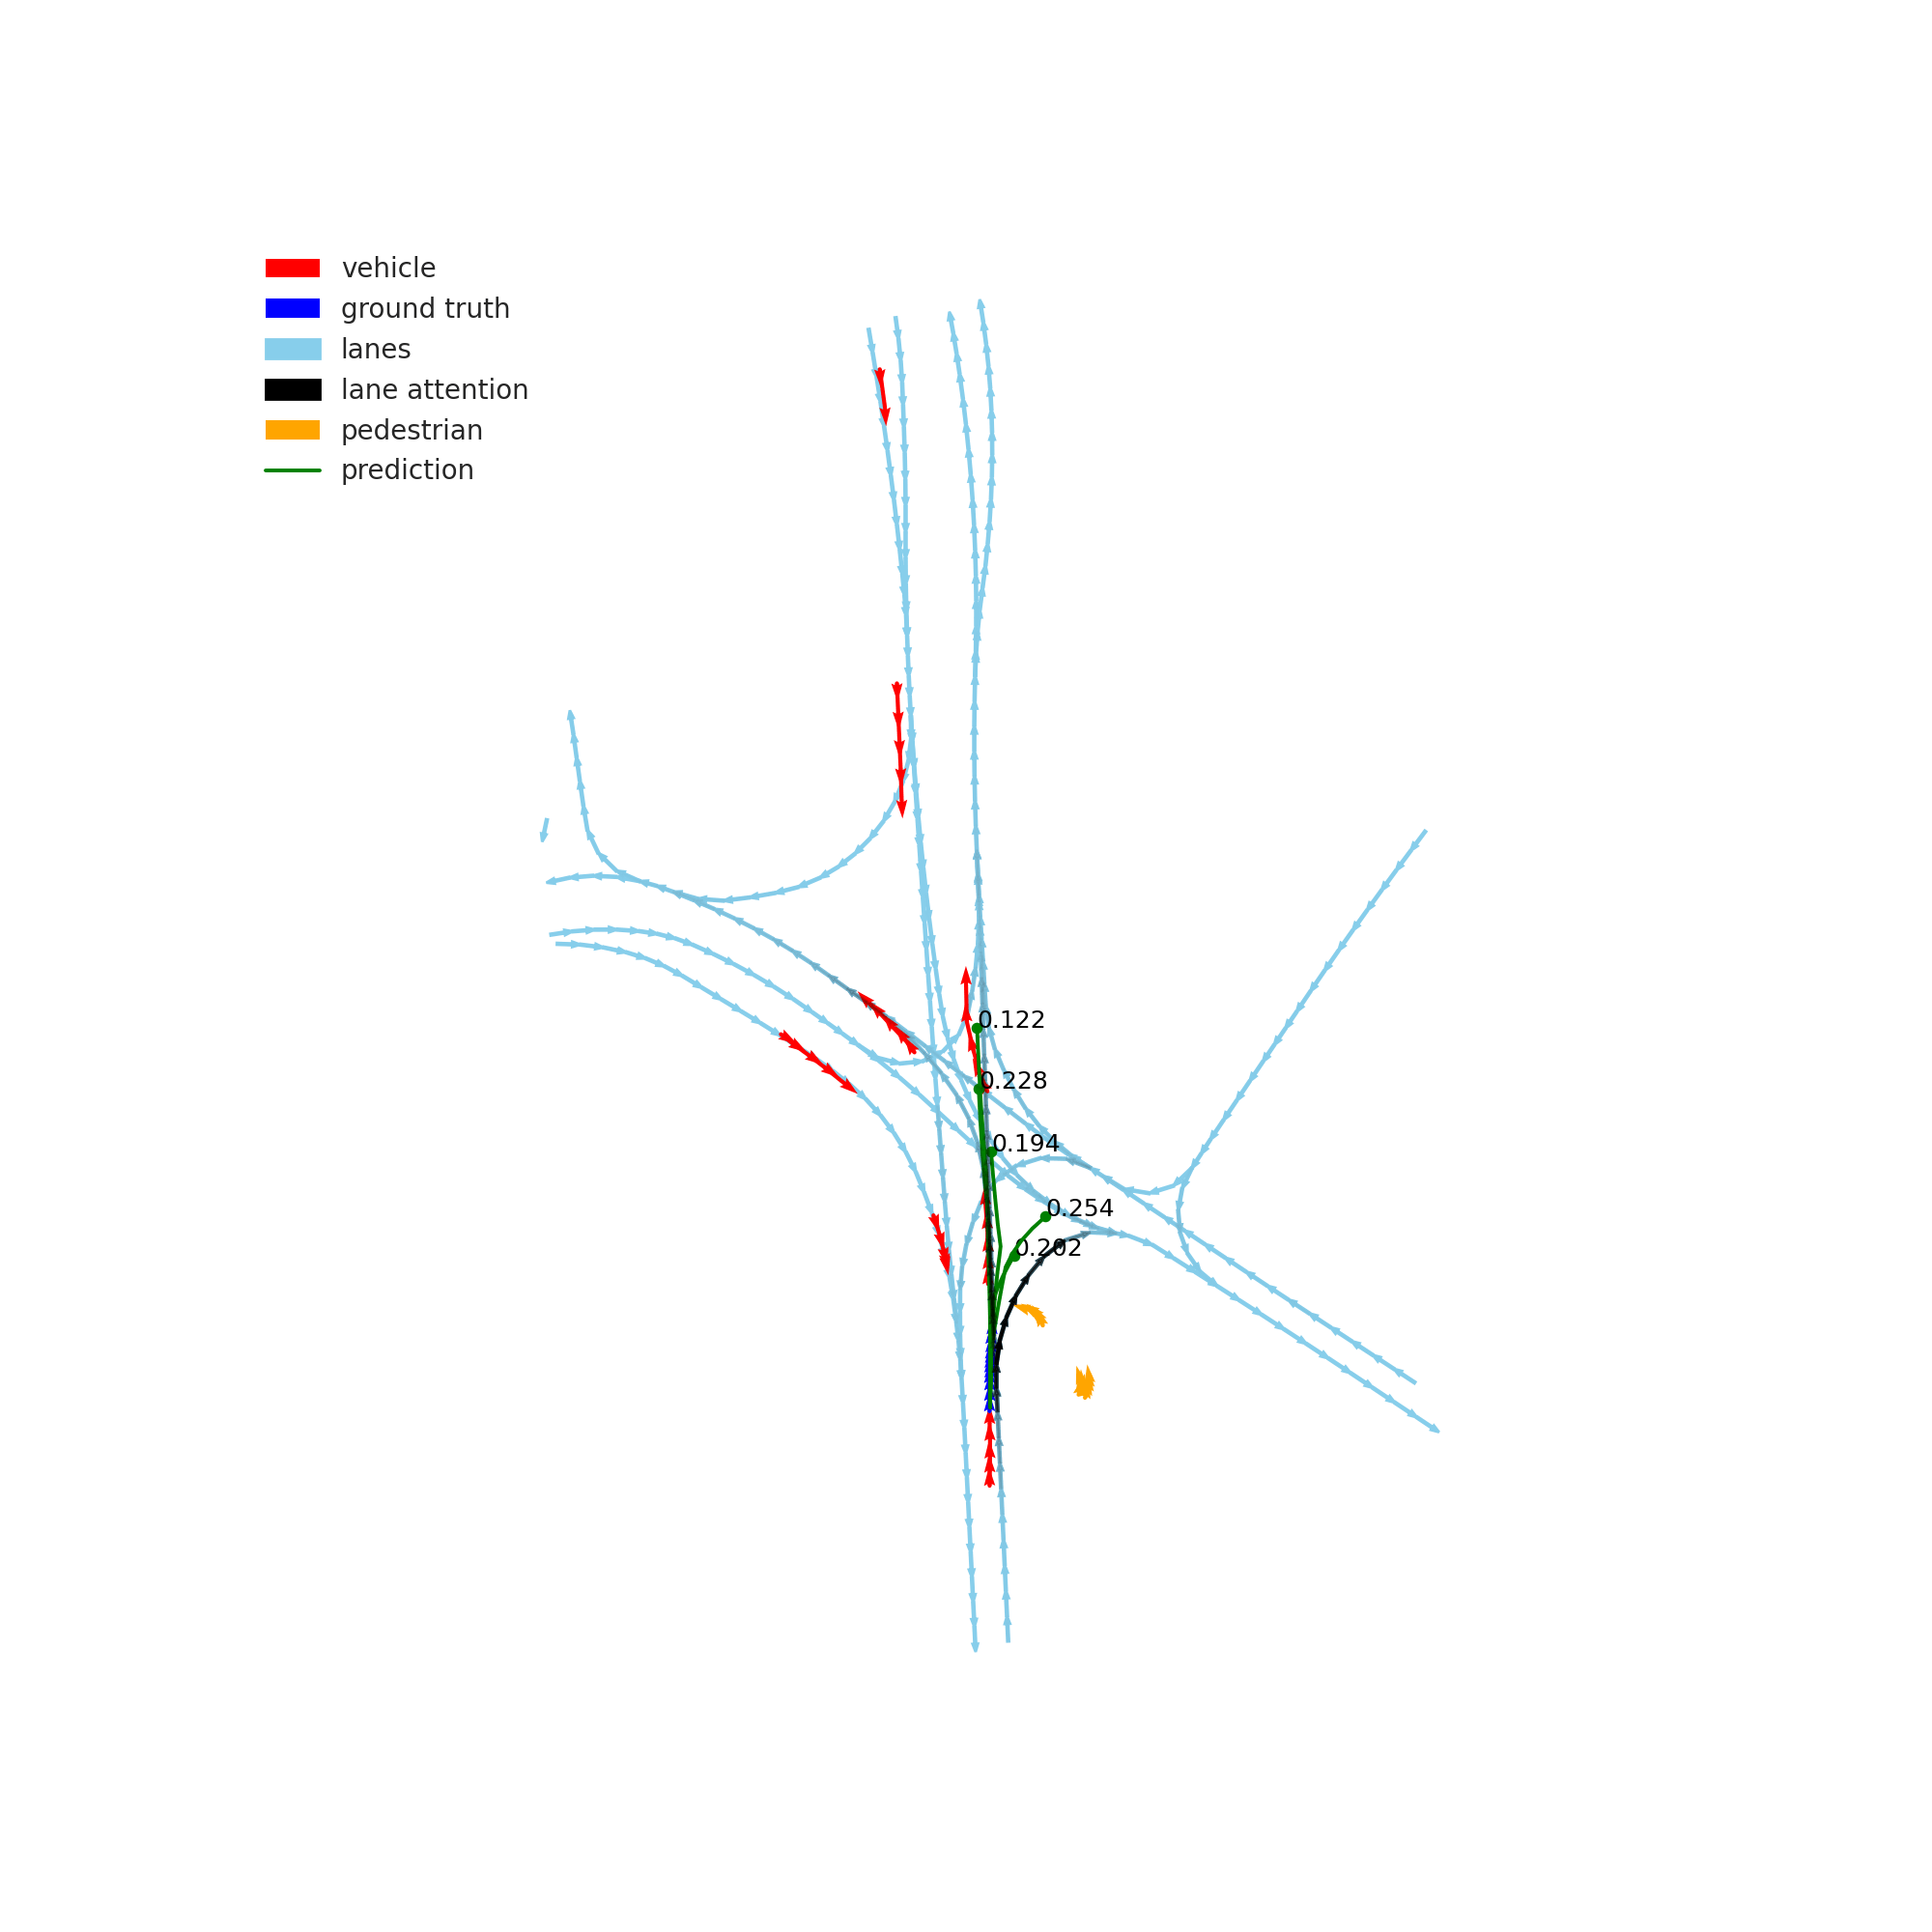
\includegraphics[height=4cm,trim={300 160 280 330},clip]{images_results/2706cc4eb61844a1a5c7a5cb766ffc2e_37ab2d88d07846ef96d5227e9c5a15d7_minADE5_5.01_0-min.png}
        \caption{Initial}
    \end{subfigure}
    \begin{subfigure}[t]{0.3\linewidth}
        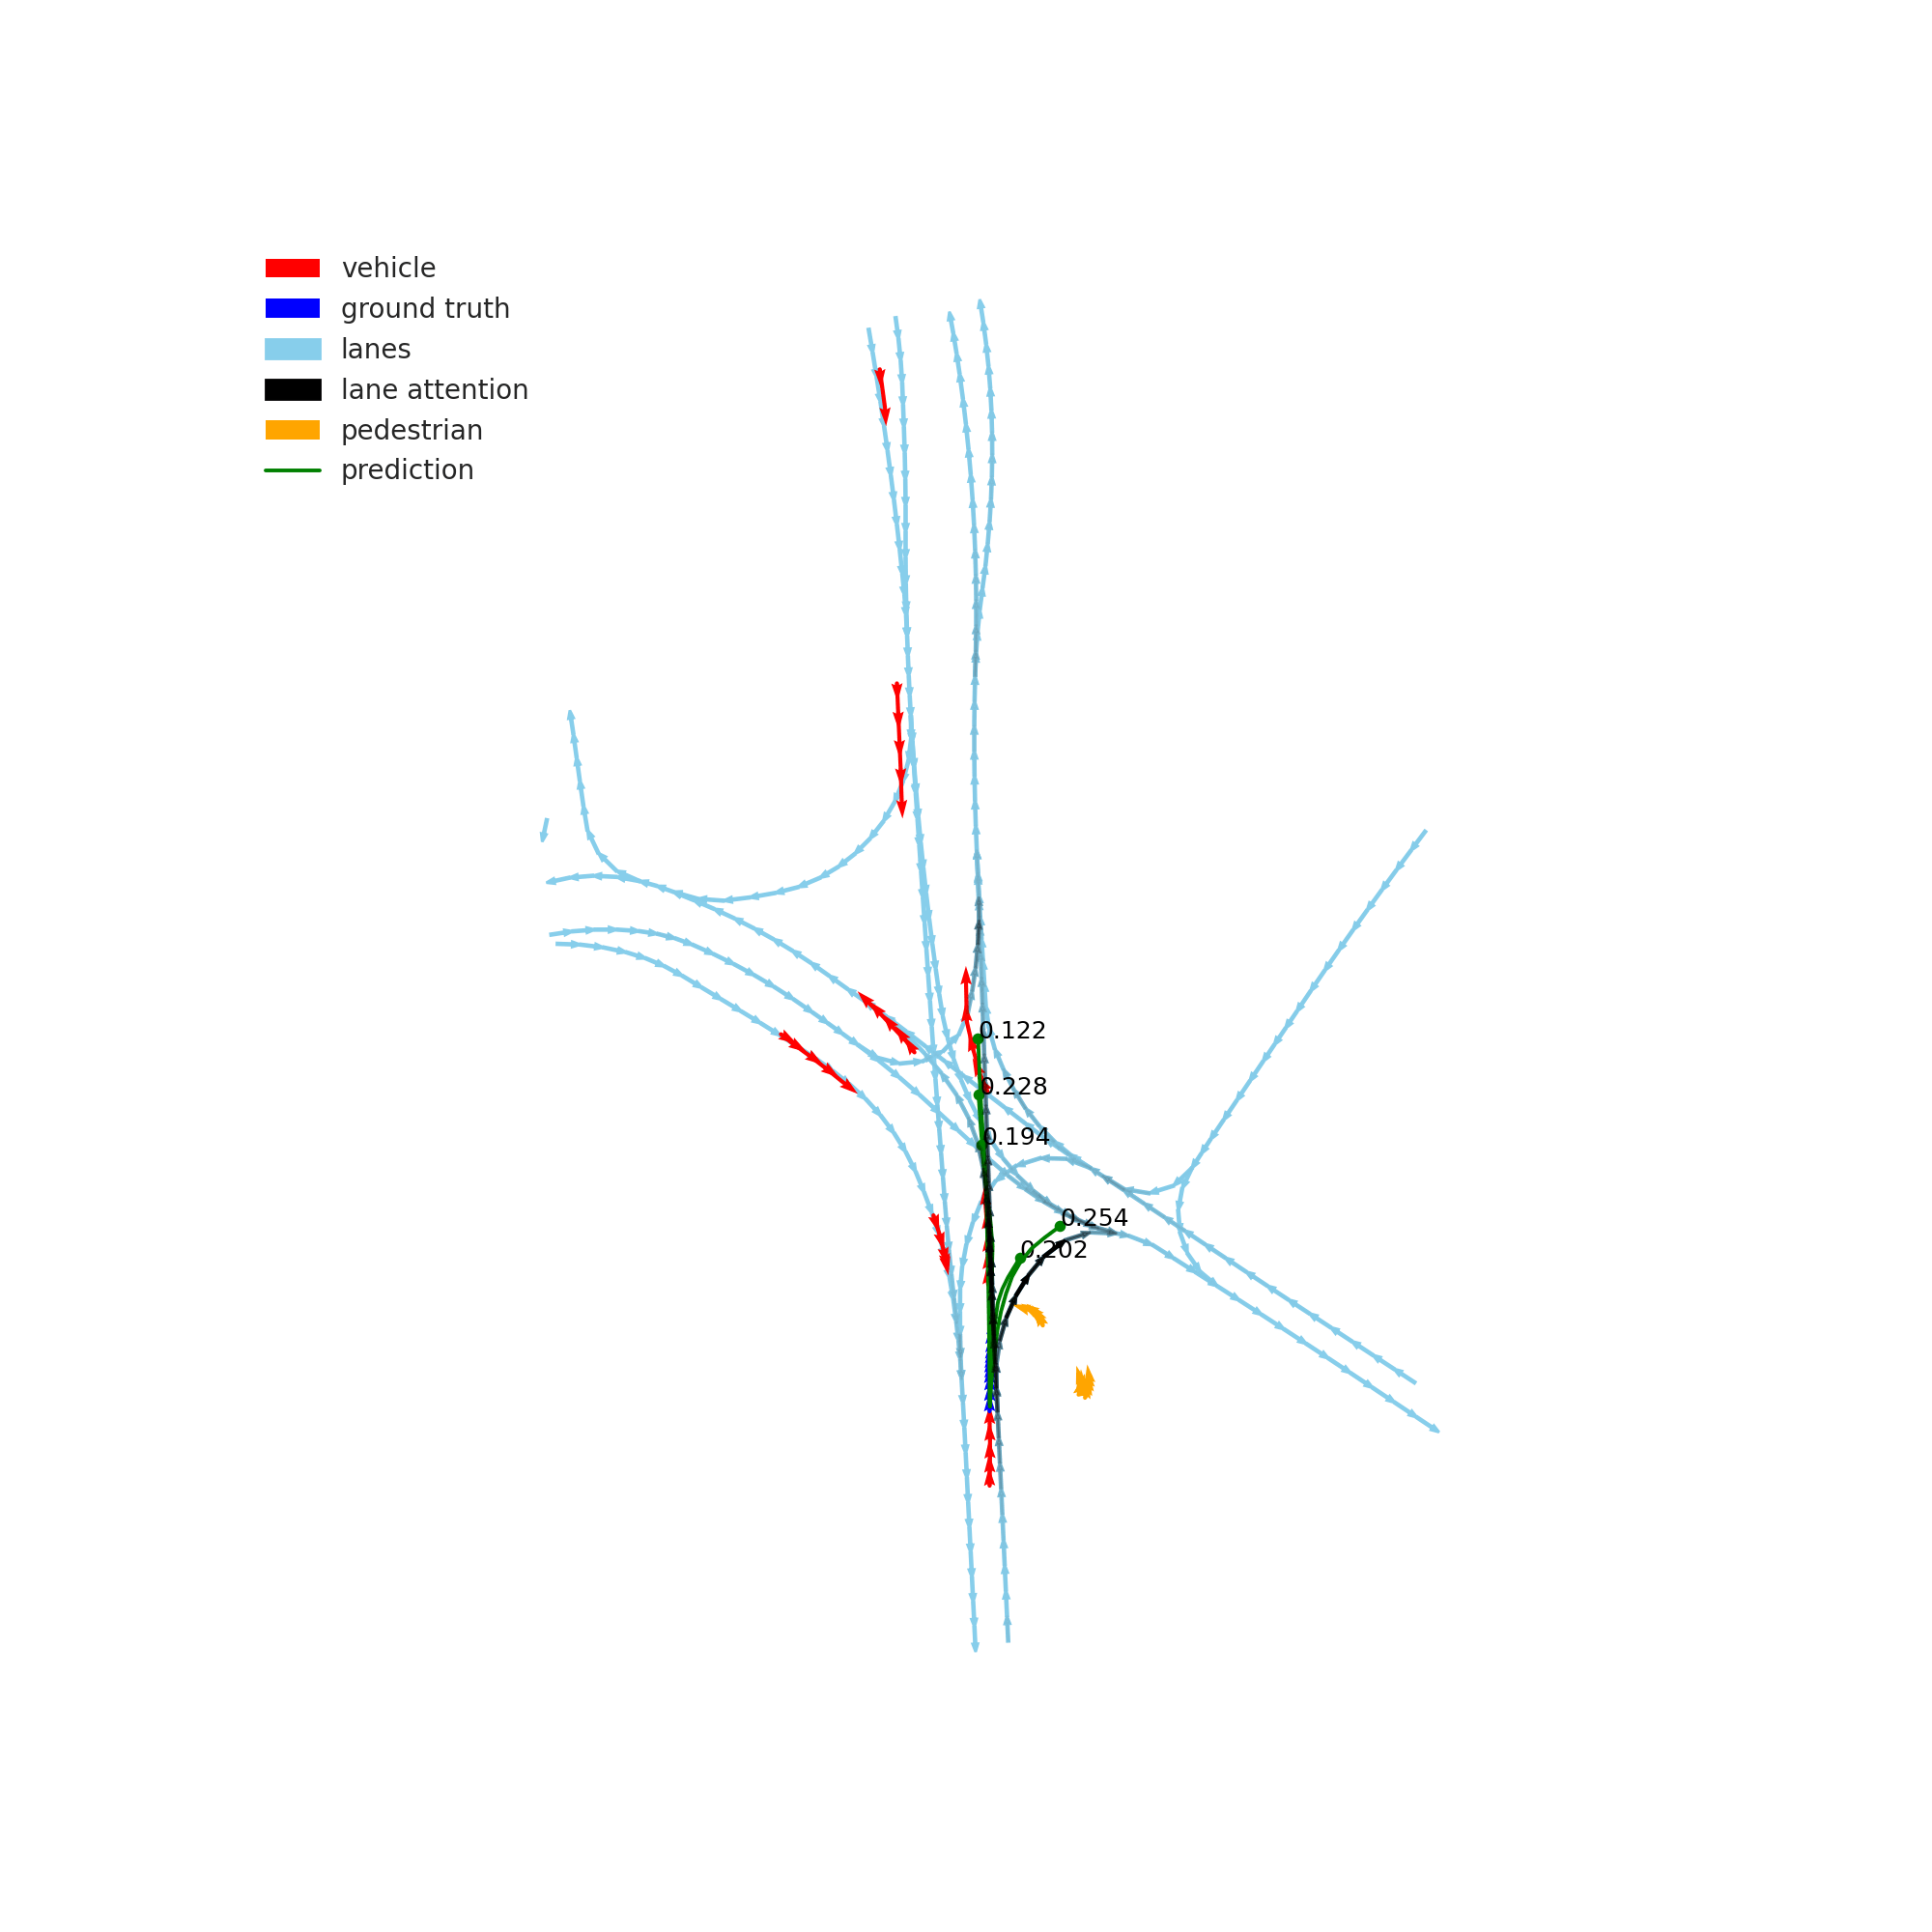
\includegraphics[height=4cm,trim={300 160 280 330},clip]{images_results/2706cc4eb61844a1a5c7a5cb766ffc2e_37ab2d88d07846ef96d5227e9c5a15d7_minADE5_5.01_1-min.png}
        \caption{Refinement}
    \end{subfigure}
    \begin{subfigure}[t]{0.3\linewidth}
        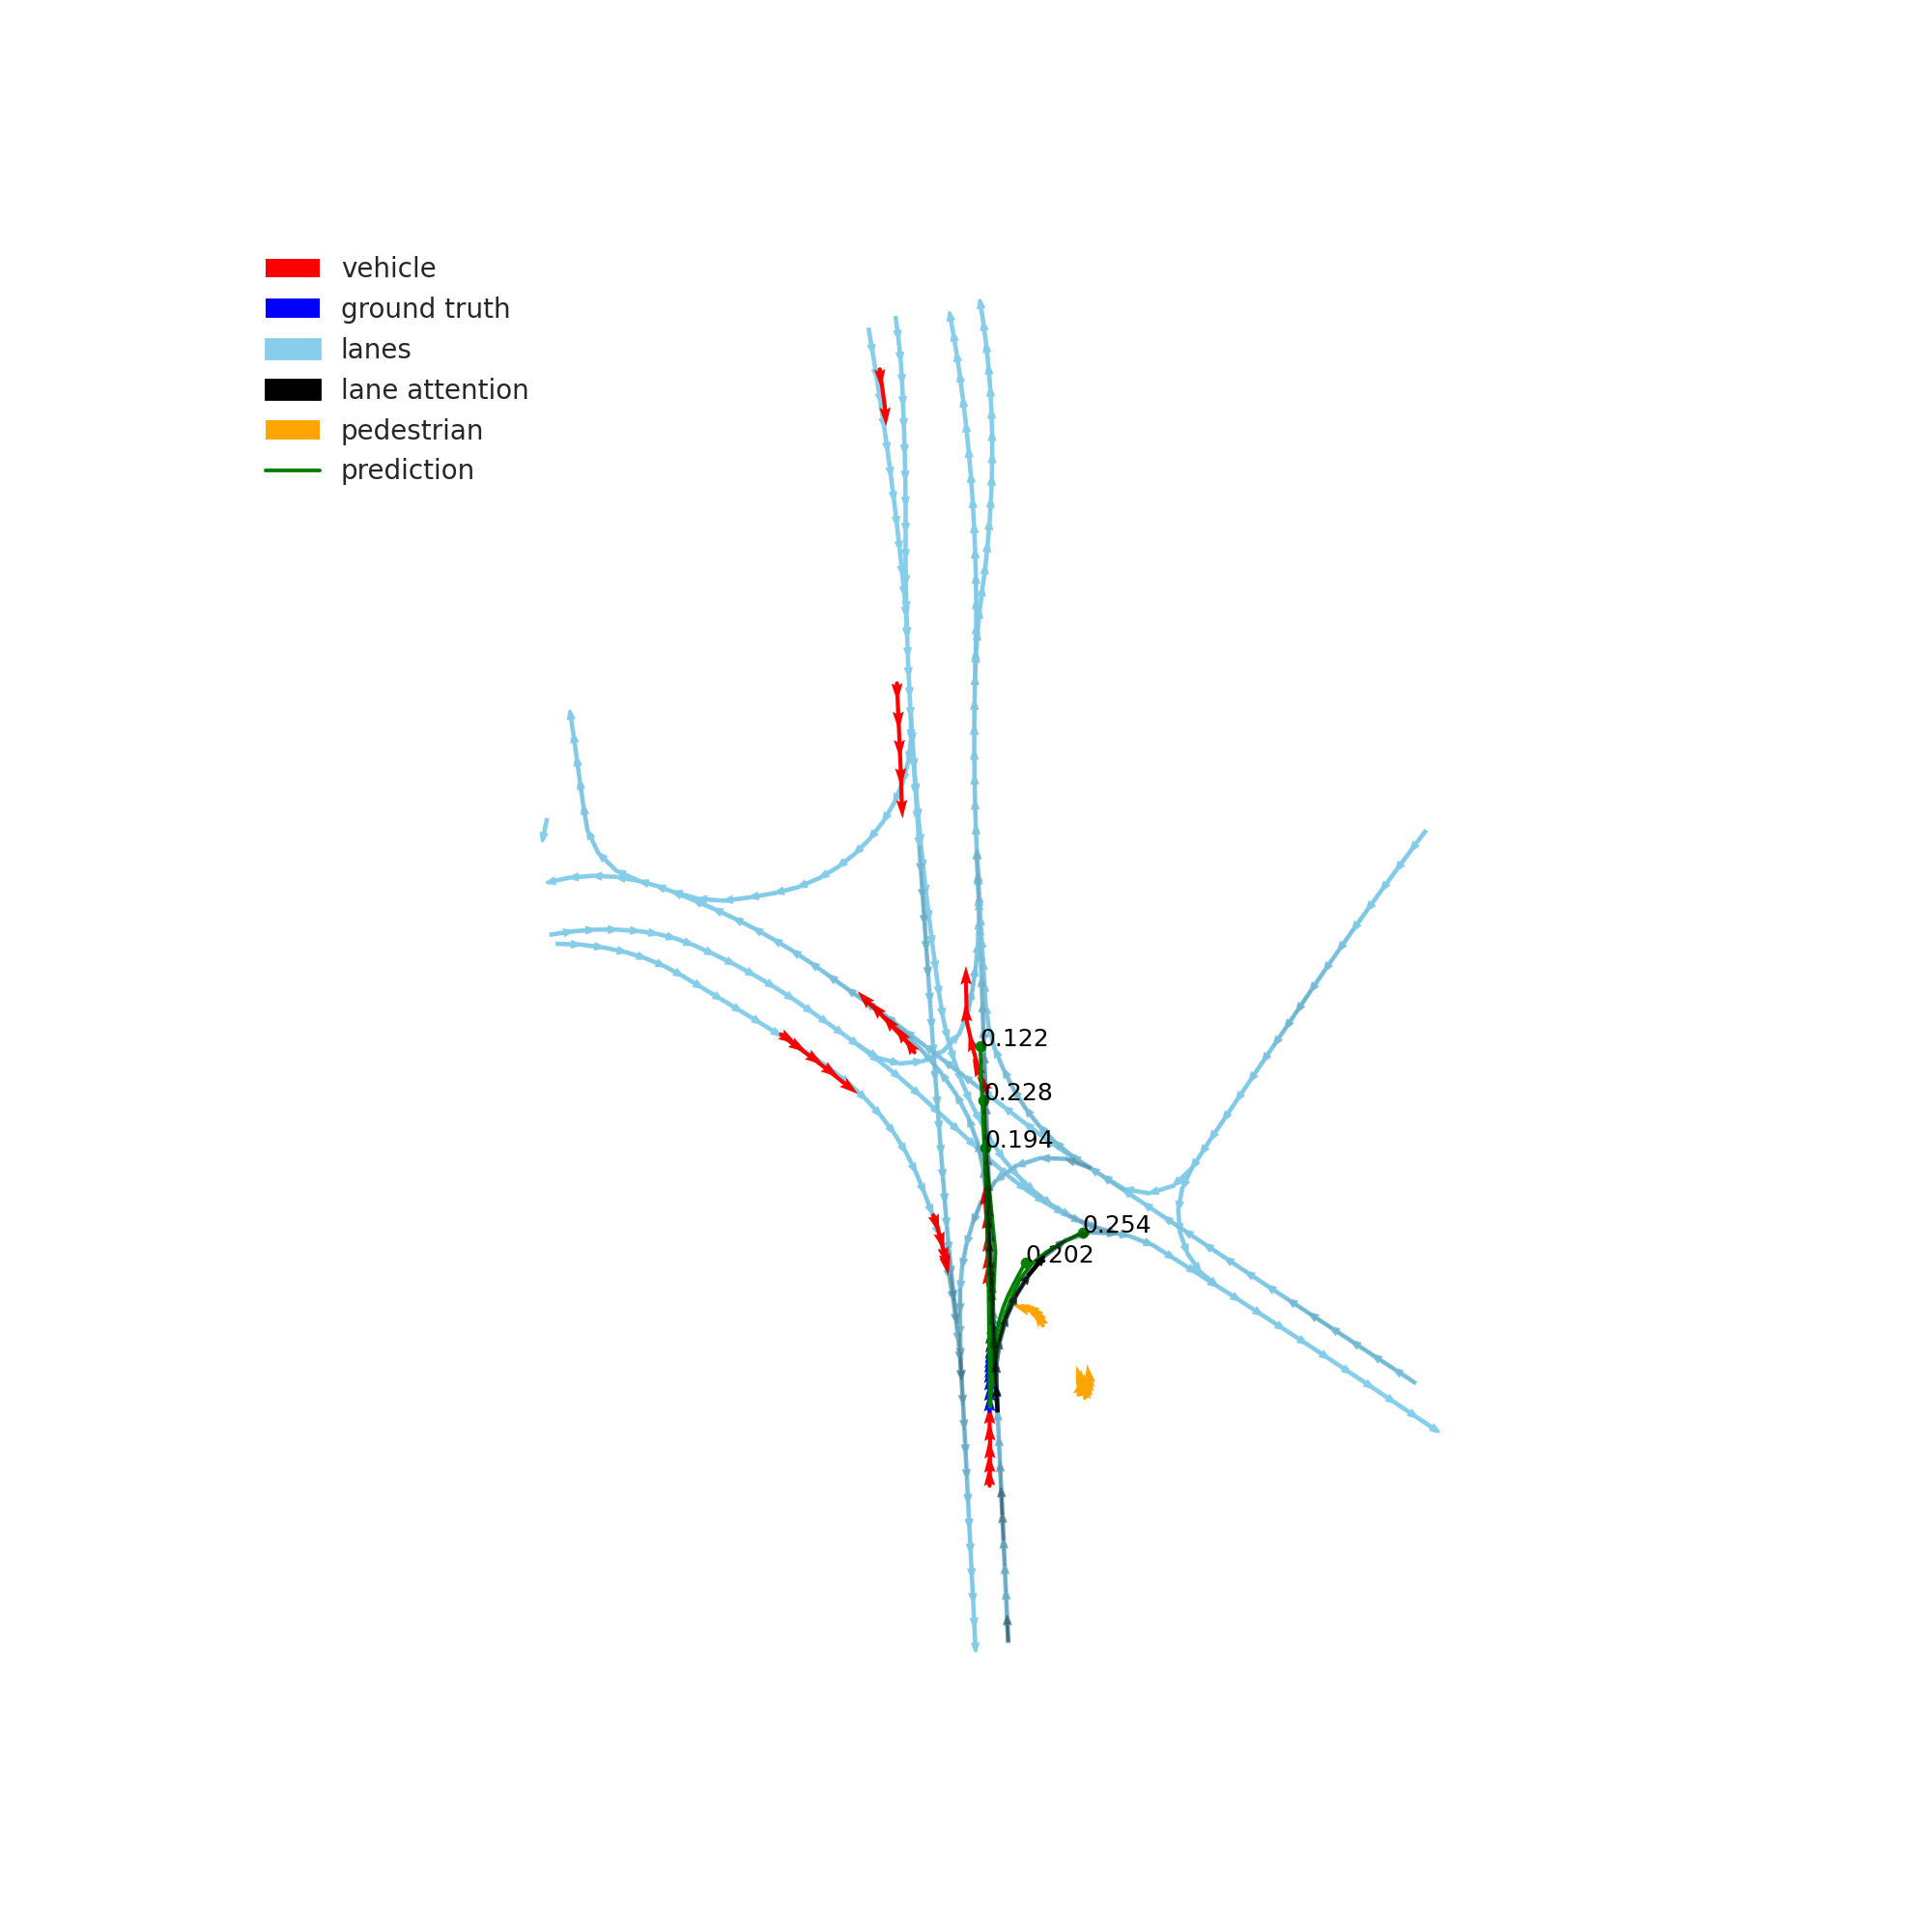
\includegraphics[height=4cm,trim={300 160 280 330},clip]{images_results/2706cc4eb61844a1a5c7a5cb766ffc2e_37ab2d88d07846ef96d5227e9c5a15d7_minADE5_5.01_2-min.png}
        \caption{Final}
    \end{subfigure}
    \begin{tikzpicture}[remember picture,overlay]
     \node at (0, 3.3)      {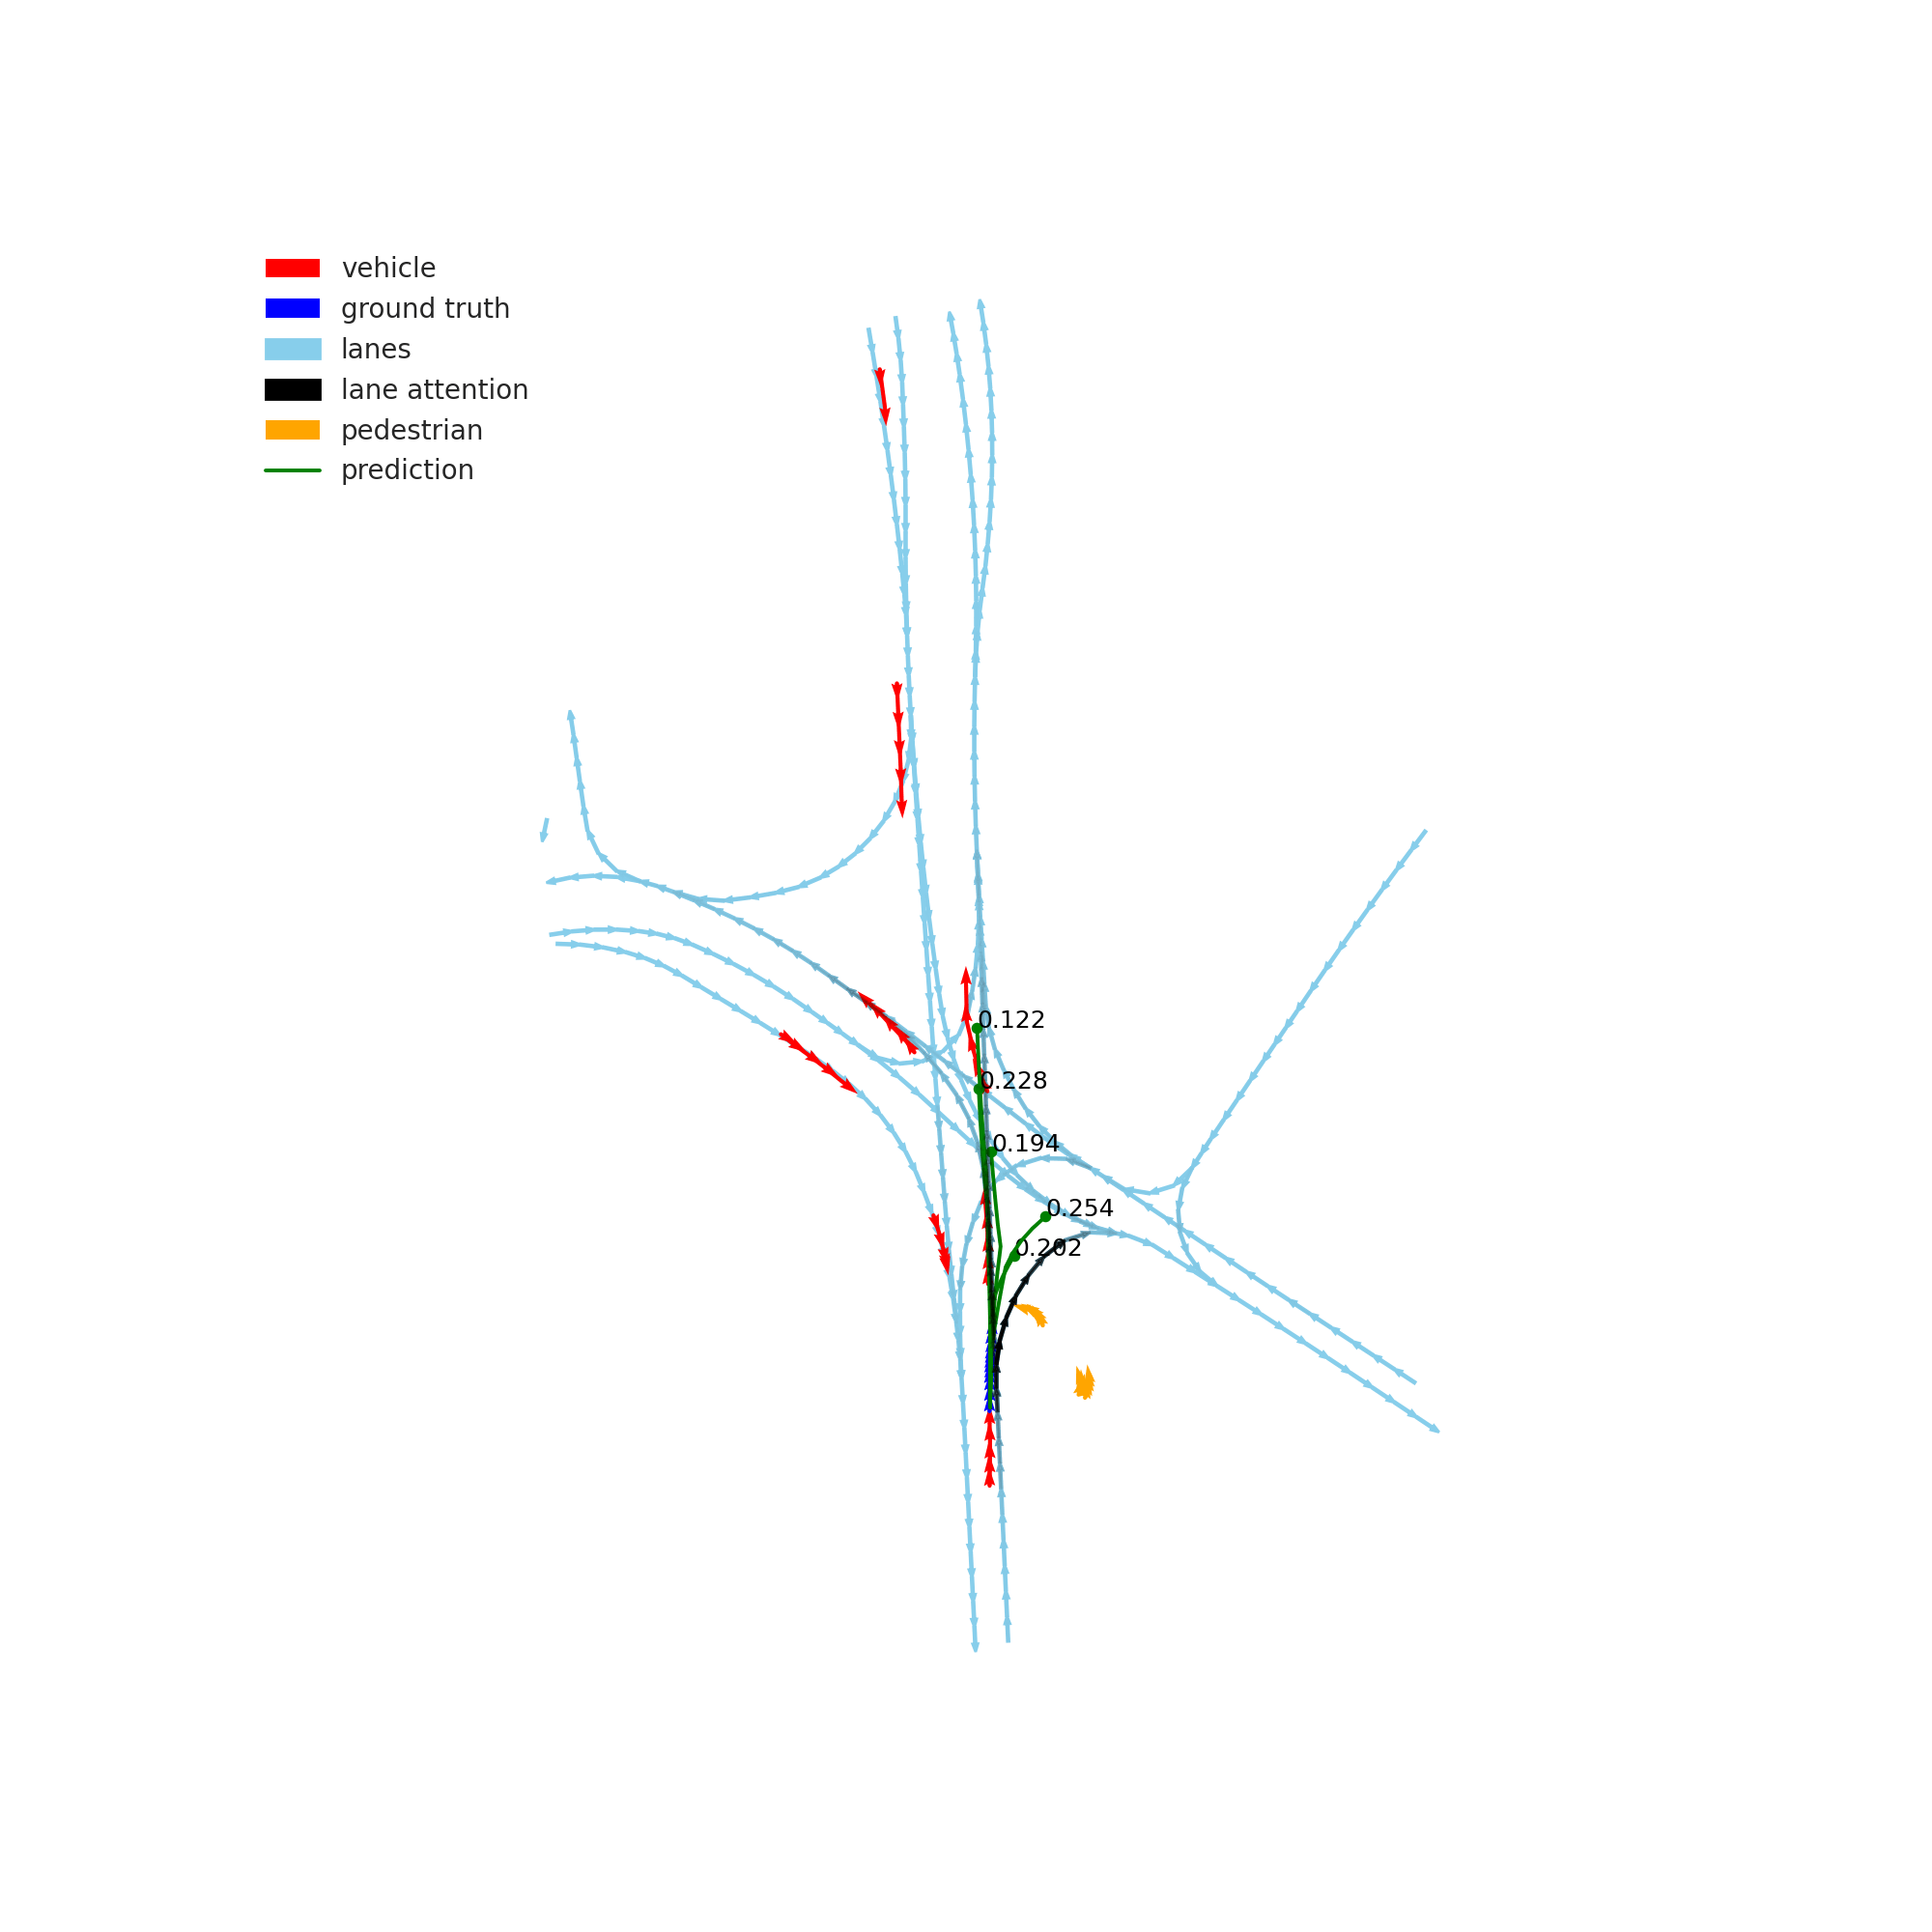
\includegraphics[width=0.23\linewidth,trim={110 500 450 85},clip]{images_results/2706cc4eb61844a1a5c7a5cb766ffc2e_37ab2d88d07846ef96d5227e9c5a15d7_minADE5_5.01_0-min.png}};
    \end{tikzpicture}
    \caption{A schematic of predicted trajectories (green) with mode probabilities for the target agent. In (a), the initial predictions exhibit noticeable misalignment with the drivable lanes. However, through iterative refinement steps, the trajectories become increasingly structured, as seen in (b) and (c). Notably, the final predictions not only align well with the road topology but also exhibit a realistic distribution of possible future paths. }
    \label{fig:nuScenes_qual}    
\end{figure}

\noindent(2) Prior studies \cite{gao2020vectornet,kim2021lapred,zhou2022hivt,wang2022ltp,liu2024laformer,ngiam2021scene,zhou2023query} fail to account for lane connection information among different lanes at intersections, lane splits and lane merges. Sun et al. \cite{sun2024semanticformer} attempt to address this limitation by generating a knowledge graph of lane segments to learn their long-range dependency. However, this approach heavily relies on map ontology, which restricts its scalability. 

\noindent(3) Predicted trajectories frequently exhibit jerky behavior and poor lane alignment. Previous studies \cite{wang2022ltp,sun2024semanticformer} address this issue by generating a large number of trajectory proposals and filtering out those deemed unreasonable. Alternatively, other works \cite{zhou2023query,liu2024laformer} employ two-stage prediction frameworks, where the first stage produces coarse trajectory anchors, and the second stage refines these anchors by calculating the corresponding offsets. However, both approaches are computationally expensive; the former due to the generation of redundant proposals and the latter due to the additional learnable parameters required for the refinement module. Zhou et al.'s adaptive refinement method \cite{zhou2024smartrefine} mitigates these costs by performing iterative refinement with minimal computational overhead. Nonetheless, its performance is highly sensitive to hyperparameter selection, limiting its robustness in real-world applications.

To address the aforementioned challenges, we propose \textbf{L}ane based \textbf{M}otion Prediction Trans\textbf{former} (LMFormer), that incorporates lane-aware attention within the cross-attention layer of the prediction module. Our method dynamically prioritizes lane segments, using them as anchors to predict future trajectories. By keeping the lengths of individual lane segments sufficiently small, we effectively capture road curvature. However, this introduces the issue of long-range dependencies across lane segments. To overcome this, we construct a graph of lane segments that captures the long-range road structure. A graph neural network (GNN)-based map encoder is employed to enrich each lane segment's representation with information from downstream segments, including lane splits and lane merges. Notably, our map encoder avoids collecting information from irrelevant or oppositely directed lane segments, as done in \cite{liang2020learning}, ensuring greater computational efficiency. We further address the challenge of cost-effective refinement by computing additional refinement losses from intermittent output queries of stacked layers. To do so, we hypothesize that the output queries of the intermittent transformer layers should map to the same latent space as the final layer. Thus, intermittent output queries can also be transformed into trajectories and compared against the ground truth. It is important to note that the weights across different stacked layers are not shared. To the best of our knowledge, no existing trajectory prediction approach leverages intermittent outputs of stacked transformer layers to compute additional refinement losses.

We validate our proposed approach through extensive experimentation on the nuScenes \cite{caesar2020nuscenes} and the DeepScenario \cite{lu2023deepscenario} datasets, achieving SOTA performance across a range of metrics. We demonstrate that:

\begin{itemize}
    \item The incorporation of lane awareness within the cross-attention layer of the transformer-based architecture enhances explainability in the prediction module.
    \item The \ac{gnn}-based architecture effectively models long-distance dependencies across lane segments and improves the accuracy of predicted trajectories.
    \item The iterative refinement strategy refines predicted trajectories with minimal additional computational cost.
    \item LMFormer can be simultaneously trained on multiple datasets to achieve better generalization capabilities.
\end{itemize}